\documentclass[paper=a4, fontsize=11pt]{scrartcl}
\usepackage[T1]{fontenc}  % proper encoding for output file
\usepackage[utf8]{inputenc}  % except UTF-8 character in source
\usepackage[english]{babel}  % set document language
\usepackage{amsmath,amsfonts,amsthm}  % math type setting
\usepackage{mhchem}  % chemical expressions
\usepackage{graphicx}  % inclue graphics
\usepackage{url}
\usepackage{caption}
\usepackage{subcaption}
\setlength\parindent{0pt} % Removes all indentation from paragraphs

% Macro to conveniently typeset chemical symbols.
\newcommand{\symb}[1]{$\,\mathrm{#1}$}


\title{Exercise 1: Rotational Spectra}
\author{Sample Solution}
\date{Effective: 15.11.2018}

%%%%%%%%%%%%%%%%%%%%%%%%%%%%%%%%%%%%%%%%%%%%%%%%%%%%%%%%%%%%%%%%%%%%%%%%%%%%%%%
\begin{document}

\maketitle

1. Calculate the absorption cross sections in the microwave spectral range for
the following molecules (Figure~\ref{fig:abs_molecules}):
\begin{itemize}
    \item HCl, ClO, CO, \symb{N_2O}, \symb{O_3}
\end{itemize}

Questions and answers:
\begin{itemize}
    \item Estimate the rotational constant $B$ for HCl and for CO.
    \begin{itemize}
      \item $B_{\mathrm{HCl}} \approx 300$\,GHz
      \item $B_{\mathrm{CO}} \approx 60$\,GHz
    \end{itemize}
    \item Why is $B$ larger for HCl than for CO?
    \begin{itemize}
        \item The reduced mass $\mu$ is larger for CO. This is caused by a
            larger molecule in general and a smaller mass difference of the
            atoms inside the molecule (see Figure~\ref{fig:reduced_mass}).
    \end{itemize}
    \item Do you have any idea why \symb{N_2O} behaves like a diatomic molecule
        --- and \symb{O_3} not?
    \begin{itemize}
      \item The angles between the atoms inside the molecule differ.
            \symb{N_2O} has flat angles and therefore momentums of inertia like
            a linear molecule ($I_A = 0, I_B = I_C$). \symb{O_3} has a more
            complex structure with differing momentums of inertia ($I_A \neq
            I_B \neq I_C$).
    \end{itemize}
    \item Calculate the reduced mass of the different molecules from the masses
        of the individual atoms. For the diatomic molecules this is trivial.
        For \symb{N_2O}, I think the appropriate mass can be found by careful
        thinking. You can ignore \symb{O_3}.
        \begin{itemize}
          \item The reduced mass $\mu$ for a diatomic molecule is given by
            $\mu = \frac{m_1\,m_2}{m_1 + m_2}$. The atomic masses of the
            relevant atoms are H\,$(1\,u)$, Cl$\,(35\,u)$, C$\,(12\,u)$,
            O$\,(16\,u)$ and N$\,(14\,u)$.  For the regarded molecules
            the reduced masses are:
              \begin{align*}
                &\mu(\mathrm{HCl}) = 0.972\,u \\
                &\mu(\mathrm{ClO}) = 10.98\,u \\
                &\mu(\mathrm{CO}) = 6.857\,u \\
                &\mu(\mathrm{N_2O}) \approx 7.5\,u
              \end{align*}
        \end{itemize}
    \item Calculate the bond length of the various molecules (except
        \symb{O_3}) from the reduced mass and the rotational constant. Verify
        your result with Google. Again \symb{N_2O} needs some extra thinking.
        \begin{itemize}
          \item For each molecule, the rotational constant $B$ can be found
            using Figure~\ref{fig:abs_molecules}.  The rotational constant
            (for frequencies) is defined as
            \begin{equation*}
              B = \frac{h}{8 \pi^2 I} \quad with \quad I = \mu r_0^2
            \end{equation*}
            The equations can be combined and solved for $r_0$ which is the
            bond length of the regarded molecule.
            \begin{align*}
               &r_0(\mathrm{HCl}) = 132\,pm \\
               &r_0(\mathrm{ClO}) = 158\,pm \\
               &r_0(\mathrm{CO}) = 111\,pm \\
               &r_0(\mathrm{N_2O}) \approx 233\,pm
            \end{align*}
        \end{itemize}
    \item Play with different temperatures. How does the rotational spectrum
        change? Can you explain the changes?
        \begin{itemize}
          \item Different temperatures lead to different distributions of
            energy states. With higher temperatures the amount of molecules
            in high energy states increases and absorption lines at higher
            frequencies get stronger. When observing very cold temperatures
            all molecules are in the lowest energy state ($i = 0$) and only
            one absorption line at the lowest frequency is left.
        \end{itemize}
\end{itemize}

% figure reduced mass
\begin{figure}[h]
  \centering
  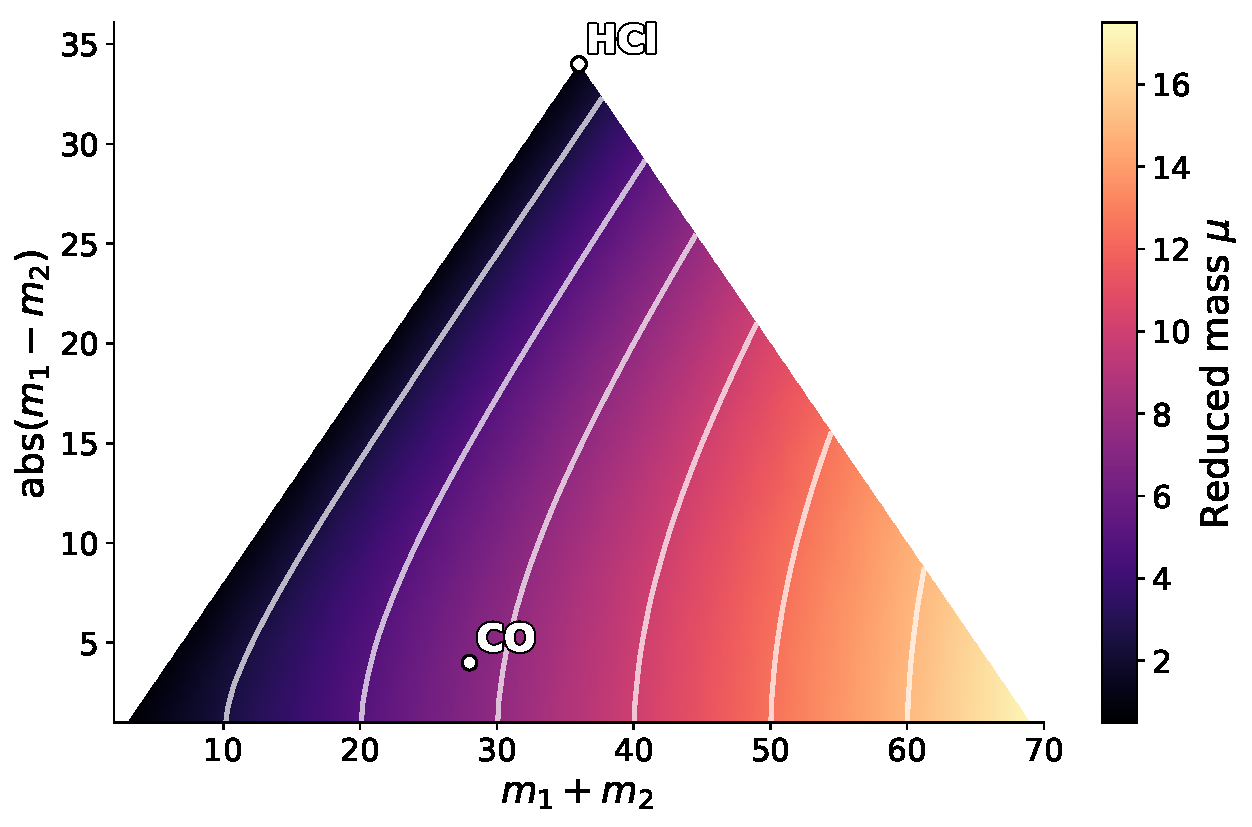
\includegraphics[width=0.75\textwidth]{plots/reduced_mass.pdf}
  \caption{Reduced mass $\mu$ as a function of total mass and mass difference.}
  \label{fig:reduced_mass}.
\end{figure}

2. Investigate other molecules!

3. Show for a diatomic molecule that the moment of inertia is given by $I = \mu r_0^2$.
\begin{equation*}
  I = \sum_i m_i r_i^2 = m_1 r_1^2 + m_2 r_2^2
\end{equation*}
The center of gravity is defined as $m_1 r_1 = m_2 r_2$. Insert this and you get
\begin{align}
  I &= m_2 r_2 r_1 + m_1 r_1 r_2 \nonumber\\
    &= r_1 r_2 (m_1 + m_2) \label{eq:a}
\end{align}
We can do more with the center of gravity equation:
\begin{align}
  m_1 r_1 &= m_2 r_2 = m_2 \overbrace{(r_0 - r_1)}^\text{from def.} = m_2 r_0 - m_2 r_1 \nonumber\\
  (m_1 + m_2) r_1 &= m_2 r_0 \nonumber\\
  r_1 &= \frac{m_2 r_0}{m_1 + m_2} \label{eq:b}\\
  r_2 &= \frac{m_1 r_0}{m_1 + m_2} \label{eq:c}
\end{align}
Insert (\ref{eq:b}) and (\ref{eq:c}) into (\ref{eq:a}):
\begin{align*}
  I &= \frac{m_2r_0 \; m_1r_0 \; (m_1 + m_2)}{(m_1 + m_2)(m_1 + m_2)} \\
    &= \frac{m_1m_2}{m_1 + m_2} r_0^2 = \mu r_0^2 \qquad\square
\end{align*}

% figures abs cross sections
\begin{figure}[ht]
    \centering
    \begin{subfigure}[t]{0.45\textwidth}
        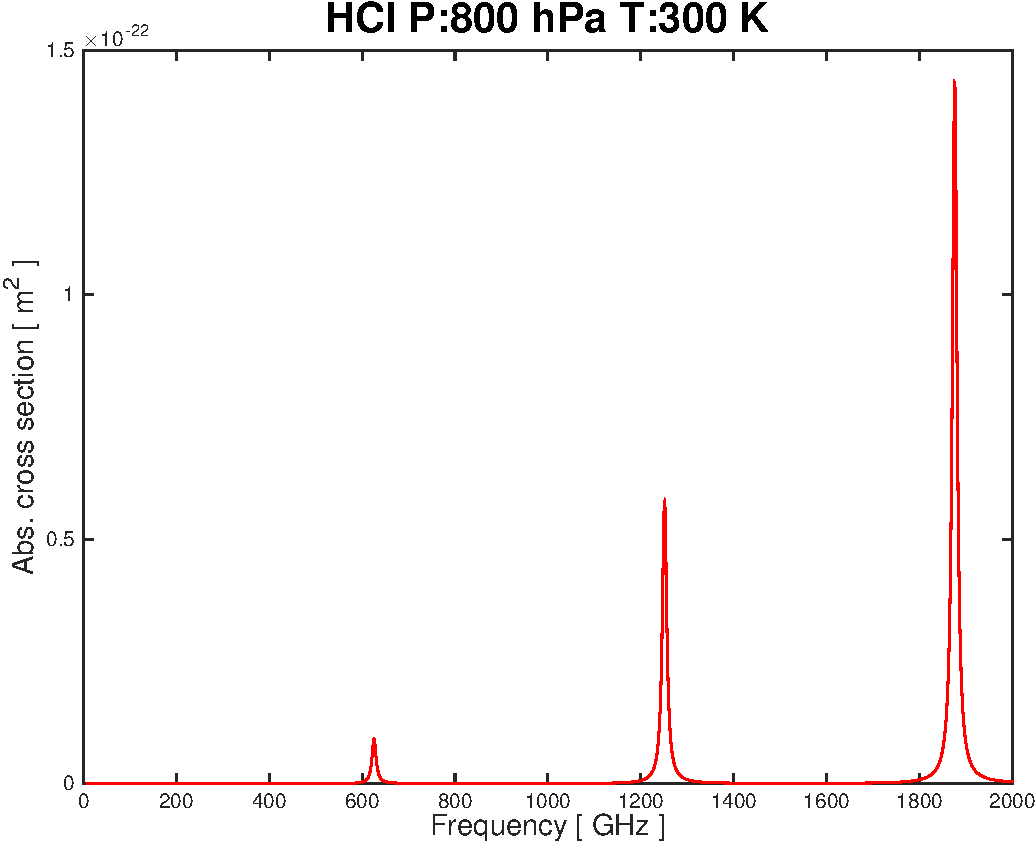
\includegraphics[width=\textwidth]{plots/plot_xsec_HCl_800hPa_300K.pdf}
        \caption{HCl}
    \end{subfigure}
    \begin{subfigure}[t]{0.45\textwidth}
        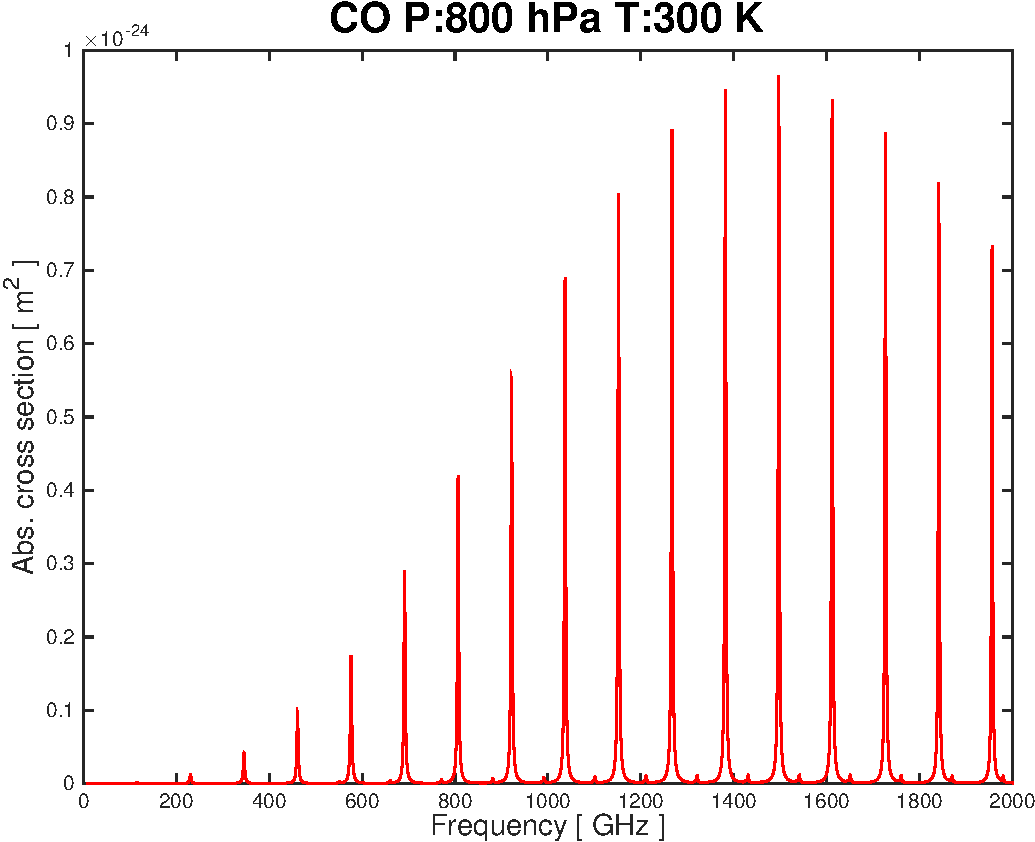
\includegraphics[width=\textwidth]{plots/plot_xsec_CO_800hPa_300K.pdf}
        \caption{CO}
    \end{subfigure}
    \begin{subfigure}[b]{0.45\textwidth}
        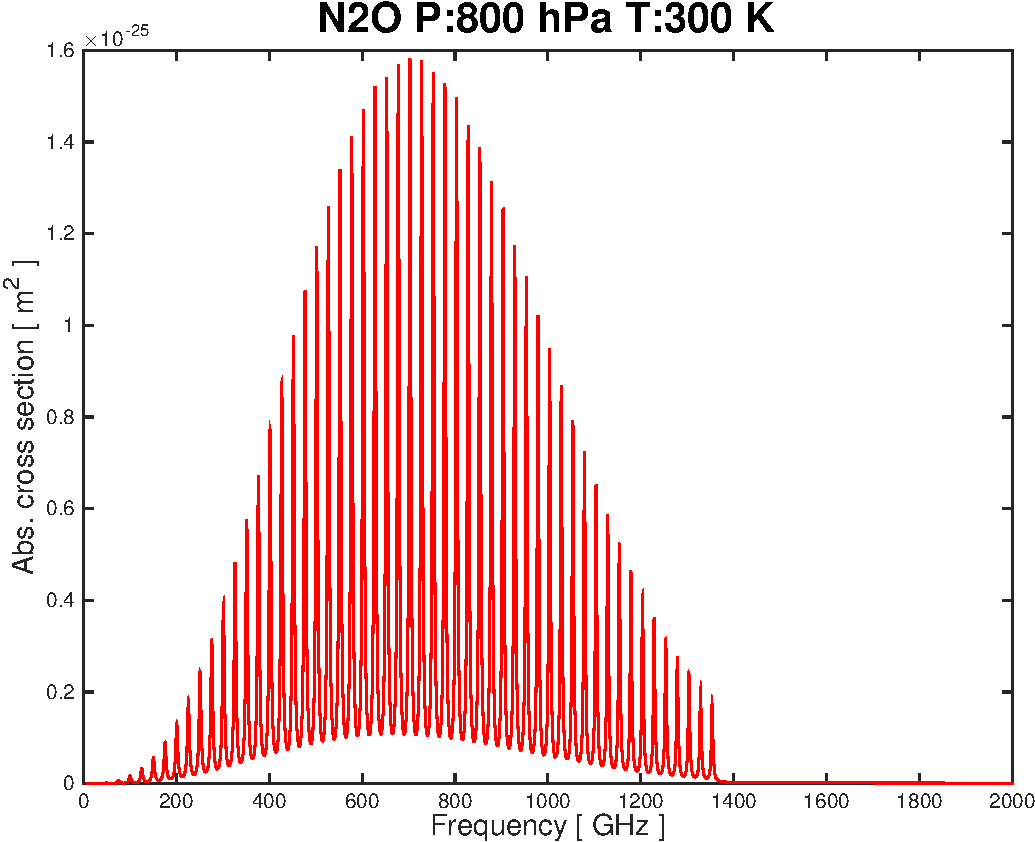
\includegraphics[width=\textwidth]{plots/plot_xsec_N2O_800hPa_300K.pdf}
        \caption{\symb{N_2O}}
    \end{subfigure}
    \begin{subfigure}[b]{0.45\textwidth}
        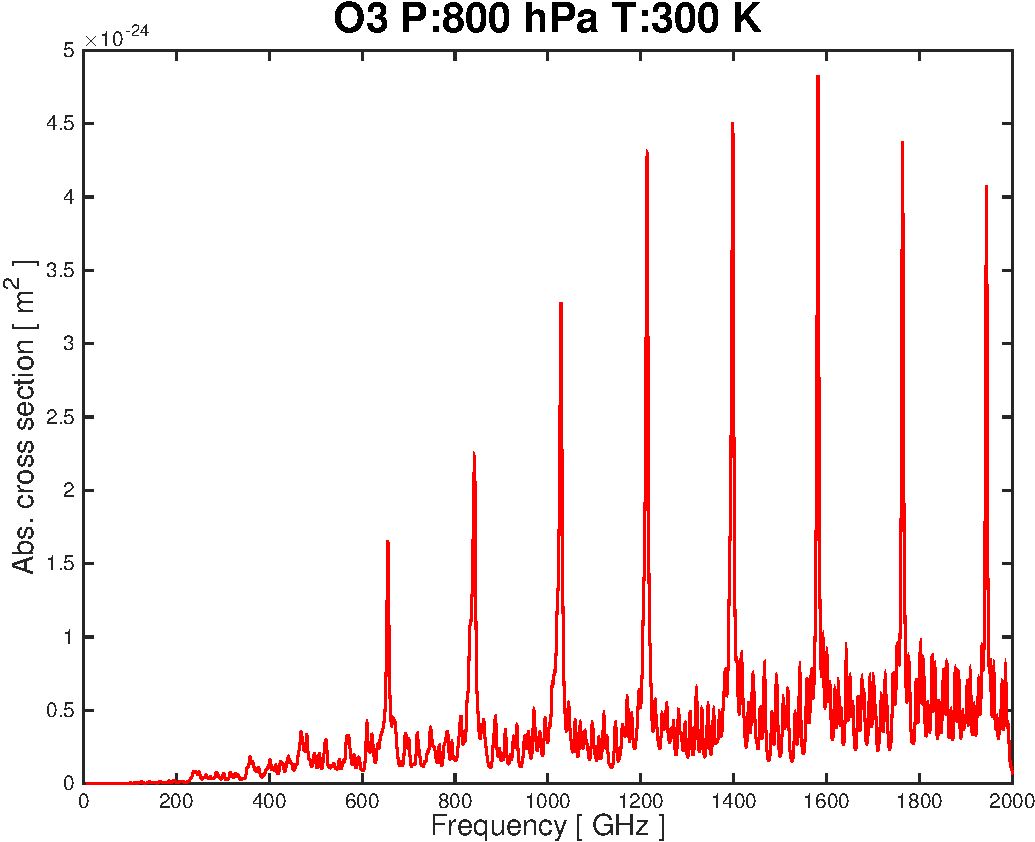
\includegraphics[width=\textwidth]{plots/plot_xsec_O3_800hPa_300K.pdf}
        \caption{\symb{O_3}}
    \end{subfigure}
    \begin{subfigure}[b]{0.45\textwidth}
        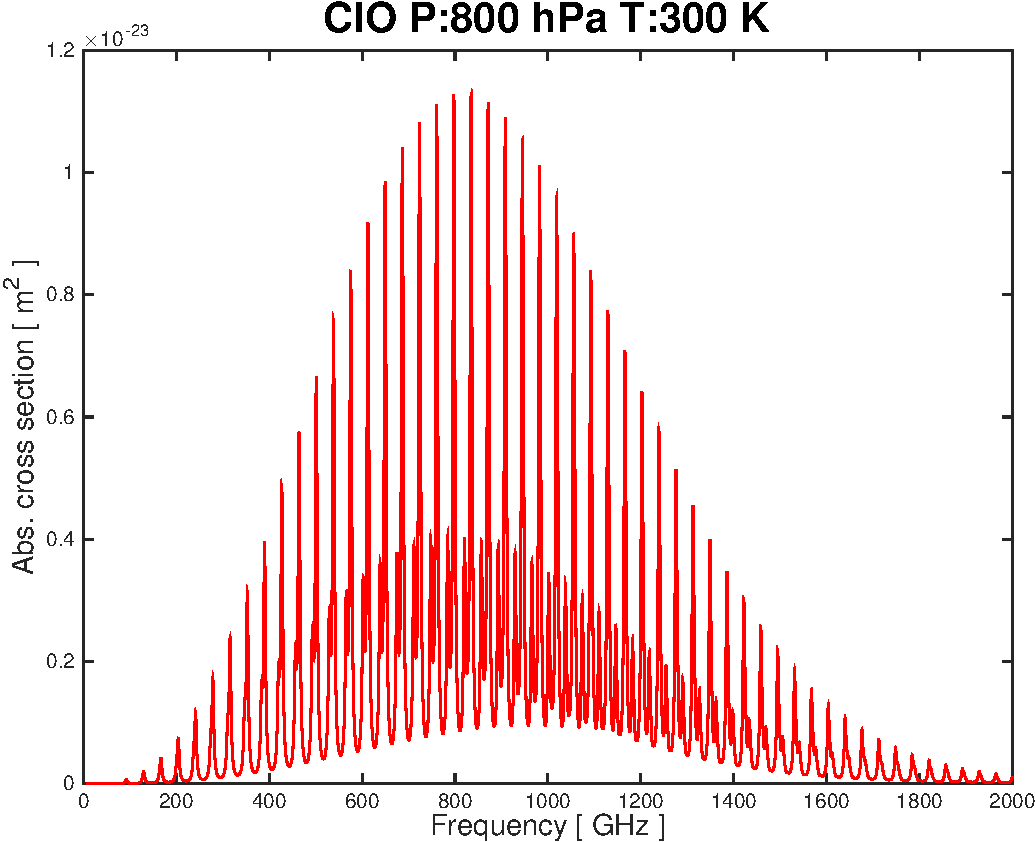
\includegraphics[width=\textwidth]{plots/plot_xsec_ClO_800hPa_300K.pdf}
        \caption{ClO}
    \end{subfigure}

    \caption{Absorption cross sections of the molecules HCl, ClO, CO,
      \symb{N_2O} and \symb{O_3}.\label{fig:abs_molecules}}
\end{figure}


\end{document}
